
\documentclass[twocolumn]{article}
\title{{\Stitlepic \vspace{1.5em}~\\ \textsc{Gesture}}\\
    \textit{\large An app to translate sign language into spoken word}}
\newcommand{\HRule}{\rule{\linewidth}{0.5mm}}
\author{\HRule \\~\\\textit{Student:} \href{http://scottsievert.com}{Scott Sievert} \hspace{5em} \textit{Advisor:} \href{http://www.ece.umn.edu/~jdhaupt/}{Jarvis Haupt}
}
\date{ }

\usepackage[left=5em, right=5em]{geometry}
\usepackage[colorlinks, linkcolor=blue, urlcolor=blue]{hyperref}
\usepackage[utf8]{inputenc}
\usepackage{array, booktabs}
\usepackage{graphicx}
\usepackage[x11names]{xcolor}
\usepackage{colortbl}
\usepackage{caption}
\newcommand{\foo}{\hspace{-0.27em}$\bullet$ \hspace{0.2em}}
\usepackage{listings}
\usepackage{amsmath, amssymb}

% "define" Scala
\lstdefinelanguage{scala}{
  morekeywords={abstract,case,catch,class,def,
    func,do,else,extends,false,final,finally,
    for,if,implicit,import,match,mixin,
    new,null,object,override,package,
    private,protected,requires,return,sealed,
    super,this,throw,trait,true,try,
    type,val,var,while,with,yield
    int,float,double
    },
  otherkeywords={[,],<,>,=,-=,=>,<-,<\%,<:,>:,\#,@},
  sensitive=true,
  morecomment=[l]{//},
  morecomment=[n]{/*}{*/},
  morestring=[b]",
  morestring=[b]',
  morestring=[b]"""
}[keywords,comments,strings]
\lstset{language=Scala}

\definecolor{mygreen}{rgb}{0,0.6,0}
\definecolor{mygray}{rgb}{0.5,0.5,0.5}
\definecolor{mymauve}{rgb}{0.58,0,0.82}

\usepackage{etoolbox}
\newtoggle{InString}{}% Keep track of if we are within a string
\togglefalse{InString}% Assume not initally in string
\newcommand*{\ColorIfNotInString}[1]{\iftoggle{InString}{#1}{\color{gray}#1}}%

\lstset{literate=%
    {"}{{{\ProcessQuote{"}}}}1% Disable coloring within double quotes
    {'}{{{\ProcessQuote{'}}}}1% Disable coloring within single quote
    {0}{{{\ColorIfNotInString{0}}}}1
    {1}{{{\ColorIfNotInString{1}}}}1
    {2}{{{\ColorIfNotInString{2}}}}1
    {3}{{{\ColorIfNotInString{3}}}}1
    {4}{{{\ColorIfNotInString{4}}}}1
    {5}{{{\ColorIfNotInString{5}}}}1
    {6}{{{\ColorIfNotInString{6}}}}1
    {7}{{{\ColorIfNotInString{7}}}}1
    {8}{{{\ColorIfNotInString{8}}}}1
    {9}{{{\ColorIfNotInString{9}}}}1
}

\lstset{ %
    backgroundcolor=\color{white},   % choose the background color; you must add \usepackage{color} or \usepackage{xcolor}
    basicstyle=\footnotesize\ttfamily,        % the size of the fonts that are used for the code
    %breakatwhitespace=false,         % sets if automatic breaks should only happen at whitespace
    %breaklines=true,                 % sets automatic line breaking
    %captionpos=b,                    % sets the caption-position to bottom
    commentstyle=\color{mygreen},    % comment style
    %deletekeywords={...},            % if you want to delete keywords from the given language
    %escapeinside={\%*}{*)},          % if you want to add LaTeX within your code
    %extendedchars=true,              % lets you use non-ASCII characters; for 8-bits encodings only, does not work with UTF-8
    frame=single,                    % adds a frame around the code
    %keepspaces=true,                 % keeps spaces in text, useful for keeping indentation of code (possibly needs columns=flexible)
    keywordstyle=\color{blue},       % keyword style
    language=Scala,                 % the language of the code
    morekeywords={*},            % if you want to add more keywords to the set
    numbers=left,                    % where to put the line-numbers; possible values are (none, left, right)
    %numbersep=5pt,                   % how far the line-numbers are from the code
    numberstyle=\tiny\color{mygray}, % the style that is used for the line-numbers
    %rulecolor=\color{black},         % if not set, the frame-color may be changed on line-breaks within not-black text (e.g. comments (green here))
    %showspaces=false,                % show spaces everywhere adding particular underscores; it overrides 'showstringspaces'
    %showstringspaces=false,          % underline spaces within strings only
    %showtabs=false,                  % show tabs within strings adding particular underscores
    stepnumber=1,                    % the step between two line-numbers. If it's 1, each line will be numbered
    %stringstyle=\color{mymauve},     % string literal style
    %tabsize=2,                       % sets default tabsize to 2 spaces
    %title=\lstname                   % show the filename of files included with \lstinputlisting; also try caption instead of title
}

\usepackage{tikz}
\usepackage{lipsum}
\newcommand*{\ClipSep}{0.4cm}


\newcommand{\Sswix}{
    \begin{figure}[t]
        \centering
        \lstinputlisting{figures/swift.scala}
        \caption{An example usage of the Swift Matrix Library.}
        \label{fig:swix}
    \end{figure}
}
\newcommand{\Sbudget}{
    \begin{figure}
        \centering
        \begin{tabular}{c | c}
            Item & Cost \\
            \hline
            Myo armbands            & \$318 \\
            Apple Developer License & \$100 \\
            Video production        & \$300 \\
        \end{tabular}
        \caption{Our project's budget.}
        \label{fig:budget}
    \end{figure}
}

\newcommand{\Stimeline}{
    \begin{figure}
        \centering
        \begin{tabular}{r |@{\foo} l}
            Completing math library & Sept -- Oct \\
            Making app work with armbands & Sept -- Nov \\
            Devising algorithm & Dec -- March \\
            Publishing results & March -- May\\
        \end{tabular}
        \caption{The proposed timeline.}
        \label{fig:timeline}
    \end{figure}
}
\newcommand{\Sscreenshot}{
    \begin{figure}
        \centering
        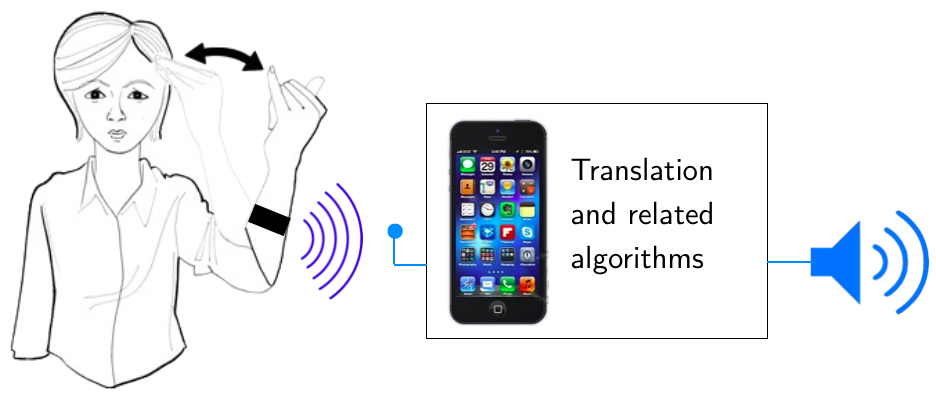
\includegraphics[width=0.4\textwidth]{figures/screenshot}
        \caption{A screenshot of an early beta version.}
        \label{fig:screenshot}
    \end{figure}
}
\newcommand{\Smyo}{
    \begin{figure}
        \centering
        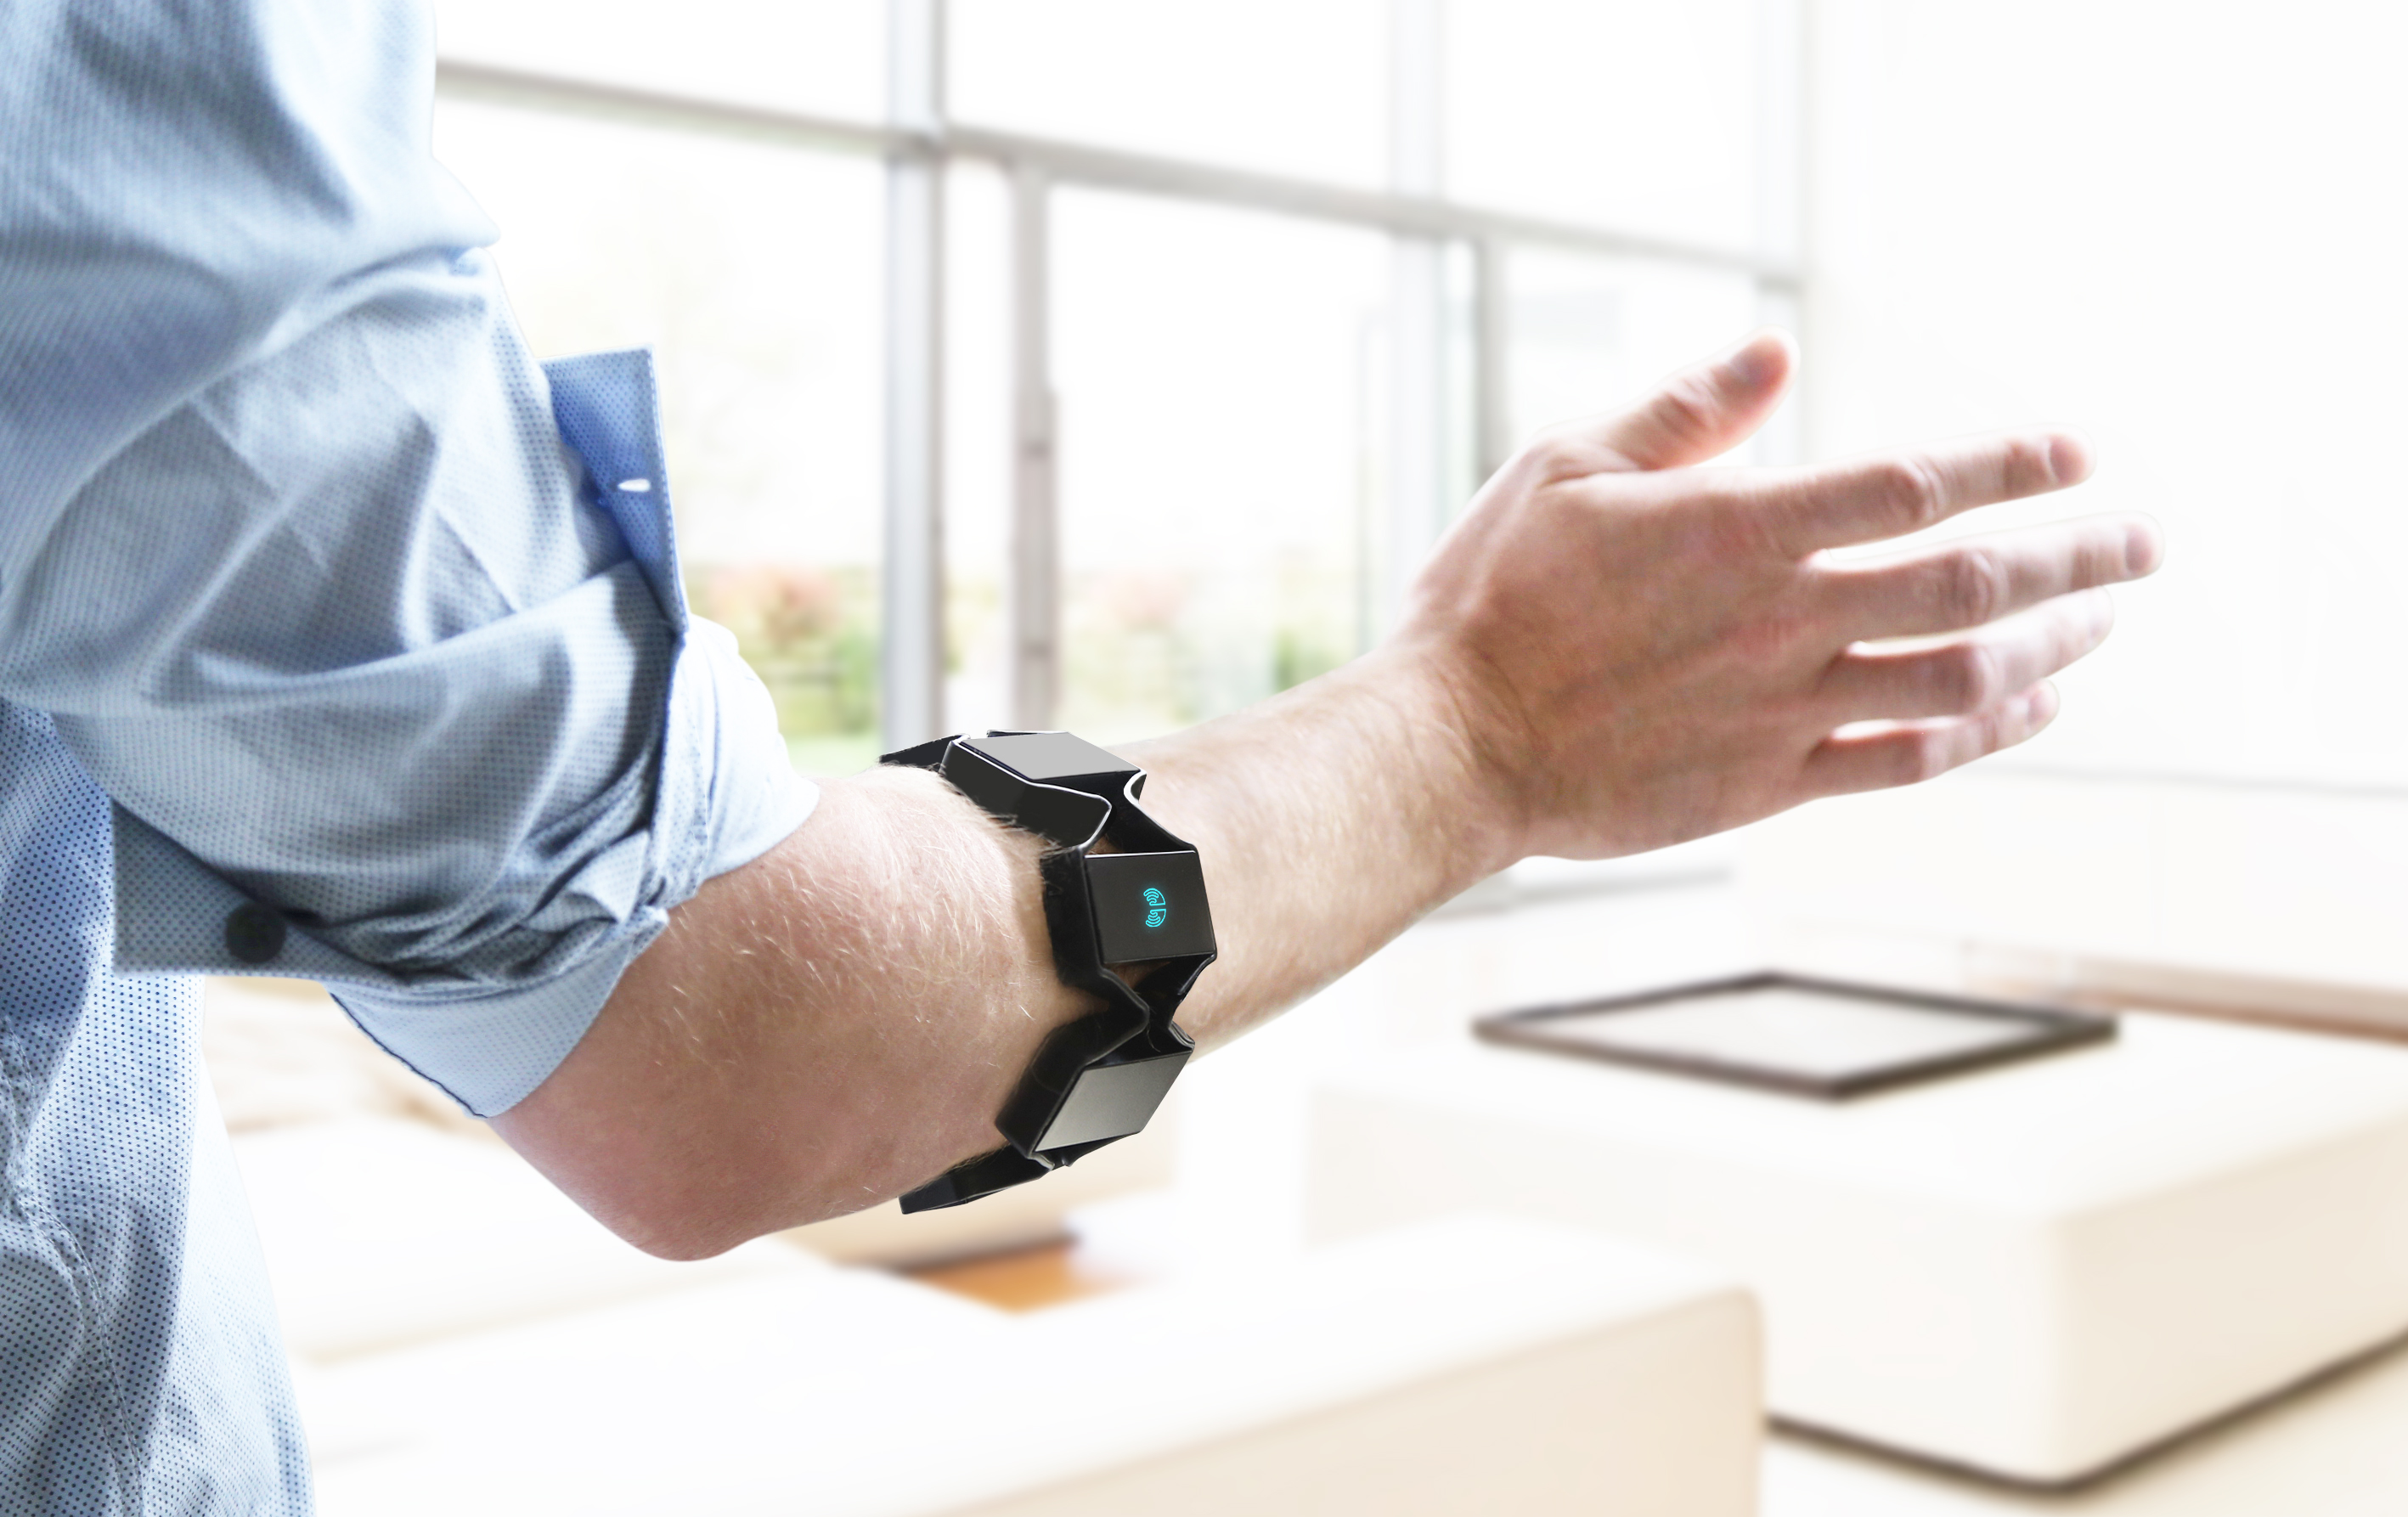
\includegraphics[width=0.4\textwidth]{figures/myo}
        \caption{The Myo armbands in use.}
        \label{fig:armbands}
    \end{figure}
}
\newcommand{\Stitlepic}{
    \begin{figure}[h]
        \centering
        \begin{tikzpicture}
        \begin{scope}
            \clip [rounded corners=.5cm] (0,0) rectangle coordinate (centerpoint) (4,4cm); 
            \node [inner sep=0pt] at (centerpoint) 
            {\includegraphics[width=4.0cm]{../../gesture/imgs/icon/icon}}; 
        \end{scope}
        \end{tikzpicture}
    \end{figure}
}



\newcommand{\system}{
    \begin{figure}
        \centering
        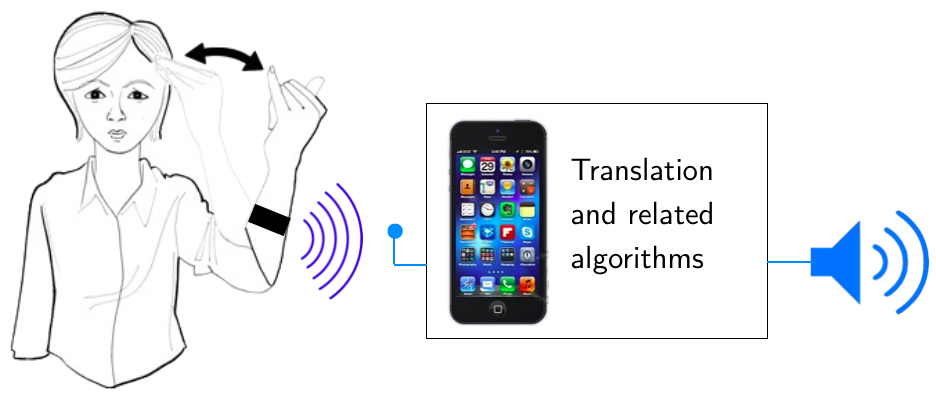
\includegraphics[width=0.4\textwidth]{figures/screenshot}
        \caption{A diagram of our project complete with armbands and smartphone app.}
        \label{fig:system}
    \end{figure}
}

\begin{document}
\begin{titlepage}
    \maketitle
    \thispagestyle{empty}
\end{titlepage}

\tableofcontents
\thispagestyle{empty}
\newpage
\listoffigures
\newpage

% outline
% backend
%   ordered armbands, talking via bluetooth
%   mention details of collecting data
%       wait for pause, collect full sentence
%   python developing
% DRC
%   involves human subjects
%   backend behind that
% research on how to handle this problem
%   NSF
%   CNNs

\abstract{
    The complete backend for our project has been developed, including communicating with both armbands simultaneously and moving data to a machine suitable for prototyping. We have cleared humans providing data with the IRB and have connected with several individuals who use ASL on a daily basis. We have a clear picture of what to do next and what algorithms to use and have installed the libraries necessary for this. The algorithm that seems to be most appropriate with certain simplifying assumptions are convolutional neural networks.
}

\section{Introduction}
This project involves translating sign language to spoken word through a smartphone app with associated hardware. A complete diagram of the system can be found in Figure~\ref{fig:system}.

\section{Backend}
Hardware is needed to obtain the data of interest and comes in the form of armbands. These armbands provide limited EMG data, acceleration and orientation data and communicate with a smartphone via Bluetooth.

To even communicate with the armbands, a smartphone app had to be developed. This smartphone app is only used to collect data and does not perform any advanced computation. The data collected is either individual signed words or a complete signed sentence.

In order to collect this data, we had to communicate with the Myo armbands via Bluetooth. This required that we conform to a third party API. These armbands are very new meaning the API is not completely stable and there were certain changes that had to be adapted to. Additionally, communicating with one armband was relatively easy and had extensive examples but communicating with two armbands had far less documentation and fewer examples.

This project is a prototype as it naturally should be and prototyping on a mobile platform is far from ideal. While the device may be capable of complex computations, it does not have other infrastructure necessary for prototyping. Capabilities to plot, easily inspect variables and rich library support are all missing on mobile platforms.

To circumvent this, we have allowed for transmission of raw data between the smartphone and computer. This is possible by writing a file to the iOS file system then using the ``File Sharing'' feature of iTunes to transfer these files across.

The language of choice while developing on a personal laptop (or possibly a server) is Python. This is a high level language similar to Matlab with similar prototyping capabilities. It is easy to visualize data or inspect variables. Additionally, Matlab and Python with their low-level libraries are roughly an order of magnitude faster then the seemingly underpowered mobile device.

It should be noted that the long term vision of this project is to eventually port this prototype to a mobile platform. The current state of technology is ready for this as it is common to carry powerful and small computing devices in pocket. However, porting this algorithm to a mobile device is in the distant future as the prototype needs to be completed.

\system

\section{Human data}
This experiment involves collecting data from humans and therefore required IRB approval. While this project does not require IRB approval, we still had to check with the IRB to ensure it didn't.

Additionally, we felt that it would be best if we obtained data from a deaf person as that is the population we're trying to help. To do this, we had to talk with the Disability Resource Center (DRC) and have linked with two deaf individuals, John Wilson and Kaity Hagen.

This process was more involved than first thought. I expected it to be simple and easy but have since learned that this process is very involved.

\section{Previous work}
At first, automatic sign language recognition (ASLR) seems similar to automatic speech recognition (ASR). Both involve computing translating some signal into text or spoken word. However, the hardware used to collect sign language data is present on 12 different channels. The algorithm behind modern ASR, the hidden Markov model (HMM) has been generalized to multiple input channels \cite{bengio2004multimodal}.

The biggest challenge in ASLR is that one sign can correspond to many different words, invalidating the assumption behind HMMs. Previous work has been done on ASLR but they had many limitations \cite{ong2005automatic}. For example, one system could effectively translate only if there were short sentences that followed a very rigid syntax.

The systems mentioned in \cite{ong2005automatic} tended to rely on speech recognition concepts, especially the algorithms of modified HMMs and neural networks. ASLR is a very difficult problem with many constraints (e.g., not ASLR to English is not 1-to-1) and accordingly the algorithms used had modifications from versions used in ASL.

\section{Next steps}
We do not want to take a giant magic step and have the entire project rest on the outcome of one algorithm. Instead, we want to take small steps and gradually improve the algorithm. As part of this, we will assume that sign language motions correspond one-to-one with spoken words. As time goes on, we hope to further expand upon this and include a more natural translation that does not make the assumption of a one-to-one translation.

Since sign language data has not been obtained, I am currently tackling a similar problem of digit recognition. Digit recognition is similar to ASLR by having multimodal inputs that can be shifted in time (or space). According to my advisor, convolutional neural networks (CNNs) are best suited for ASLR because CNNs are shift invariant.

For CNNs to be fast to be effective and require use of the GPU and low level mathematical libraries and just-in-time compiled functions. This requires that a third party library is used. Several libraries and languages were looked at including \href{https://en.wikipedia.org/wiki/Torch_(machine_learning)}{Torch7} (Lua), \href{http://caffe.berkeleyvision.org}{Caffe} (Matlab/Python) and \href{http://www.deeplearning.net/software/theano/}{Theano} (Python). I attempted to install all of these libraries and eventually settled on \href{http://theanets.readthedocs.org/en/latest/}{Theanets}, a library built on top of Theano that can also include other customization as necessary.

The first small step is to use this library to classify the handwritten digits using CNNs, a problem similar to ASLR through matrix inputs and shift-invariance necessity. This will also ensure that the library is practical for our purposes. This is currently being developed.

\section{Timeline and budget updates}
There are no updates to the budget.

The backend is done and work on the algorithm will begin. We expect this to be done in mid-April with time enough to polish the end result and write the final report.

\section{Conclusion}
The entire backend for this project has been developed. Both armbands can be communicated with simultaneously via an iOS app, the information can be transferred from iOS to a local machine for prototyping purposes and we have connected with individuals who use ASL on a daily basis.

The developed product will be a prototype and only demonstrate ASLR. The final product will likely be further polished and presented as a mobile app. This will not be a trivial undertaking and will require significant time and effort to port the algorithm of choice to the mobile platform.

\bibliographystyle{plain}
\bibliography{refs}

\end{document}
